\section{Anforderungen}

\subsection{Allgemeine Beschreibung}

\subsubsection{Produktperspektive}


\subsubsection{Produktfunktionen}


\subsubsection{Benutzer Charakteristik}


\subsubsection{Einschränkungen}



\subsection{Use Cases}

\subsubsection{Use Case Diagramm}
\begin{minipage}{\textwidth}

\begin{figure}[H]
	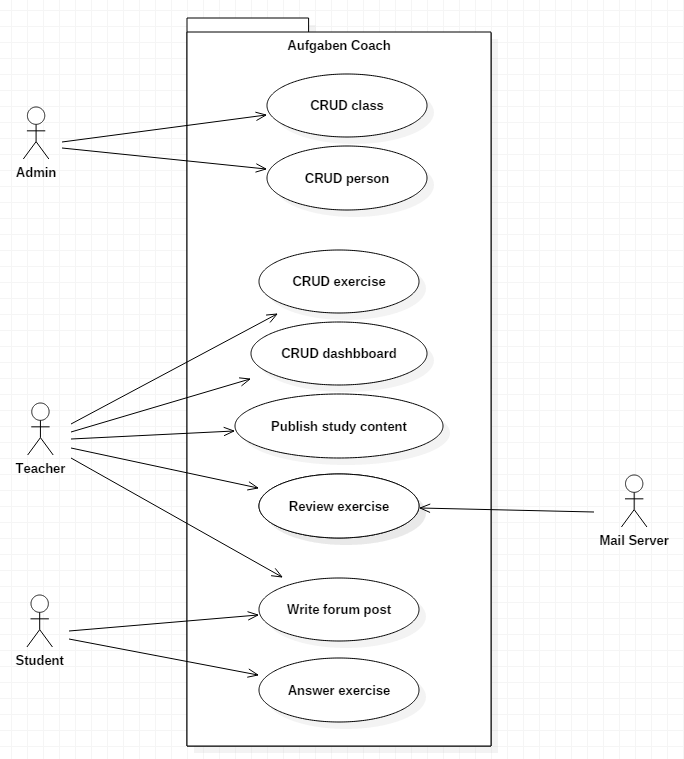
\includegraphics[width=\textwidth, height=\textheight, keepaspectratio]{images/UseCaseDiagramm.png}
	\caption{Use Case Diagramm}
\end{figure}

\end{minipage}


\begin{tabular}{| p{1cm} | p{1.3cm}|}
	\hline
	\textbf{Farbe} & \textbf{Priorität} \\
	\hline	
	grün & hoch \\
	\hline
	orange & tief \\
	\hline
\end{tabular}


\subsubsection{Aktoren}
Beschreibung der einzelnen Aktoren.
\newline
\begin{tabularx}{\textwidth}{| X | X |}
	\hline
		\textbf{Aktor} & \textbf{Beschreibung} \\
	\hline
		Administrator & Der Administrator ist für die Verwaltung der Klassen, Lehrer und Schüler zuständig. Er kann Klassen erstellen, Lehrpersonen und Schüler den Klassen zuweisen, etc. \\
	\hline
		Lehrer & Der Lehrer verwaltet die ihm zugewiesenen Klassen. Er kann Aufgaben erstellen und diese der Klasse zuweisen. Zusätzlich kann er Statistiken einsehen, die ihn über den aktuellen Wissensstand der Klasse informieren. \\
	\hline
		Schüler & Die Schüler haben Zugriff auf eine Wissensdatenbank und können Aufgaben und Quizzes, die ihnen zugewiesen wurden lösen. \\
	\hline
\end{tabularx}


\subsubsection{Beschreibung der Use Cases}

\textbf{UC01: CRUD class} Der Administrator kann Klassen erstellen, diese bearbeiten und den Klassen Lehrpersonen und Schüler zuweisen.

\begin{tabularx}{\textwidth}{| X | X |}
	\hline
		\textbf{Primärer Aktor} & Administrator \\
	\hline
		\textbf{Vorbedingung} & - \\
	\hline
		\textbf{Nachbedingung} & Die zu erstellende Klasse wurde erstellt und die zugewiesenen Personen sind ihr zugewiesen. Die zu löschende Klasse wurde entfernt. \\
	\hline
		\multicolumn{2}{|c|}{\textbf{Hauptszenario}} \\
	\hline
		\textbf{Aktor} & \textbf{System Verantwortlichkeiten} \\
	\hline
		\textbf{Klasse erstellen}
		\begin{enumerate}
			\item Der Administrator klickt auf der Adminseite auf den Button ''Neue Klasse''.
			\item Das Eintrittsjahr und der Klassenname werden gewählt und die Eingaben gespeichert.
		\end{enumerate}
		
		\textbf{Klasse bearbeiten}
		\begin{enumerate}
			\item Der Administrator klickt auf der Adminseite auf die zu bearbeitende Klasse.
			\item Auf der erschienenen Seite, können der Klasse nun Lehrpersonen und Schüler zugewiesen werden.
		\end{enumerate} 
		
		\textbf{Klasse löschen}
		\begin{enumerate}
			\item Der Administrator klickt auf der Adminseite auf das ''X'' rechts neben der zu löschenden Klasse.
		\end{enumerate} 
			& 
		\textbf{Klasse erstellen}
		\begin{enumerate}
			\item Das System erstellt die Klasse mit den angegebenen Daten.
		\end{enumerate} 
		
		\textbf{Klasse bearbeiten}
		\begin{enumerate}
			\item Das System hat die gewählten Personen der Klasse zugewiesen, oder diese entfernt.
		\end{enumerate}		
		
		\textbf{Klasse löschen}
		\begin{enumerate}
			\item Das System entfernt die Klasse aus dem System.
		\end{enumerate}	
		\\
	\hline
		\textbf{Auftrittswahrscheinlichkeit} & mittel \\
	\hline
\end{tabularx}


\textbf{UC02: CRUD person} Der Administrator kann Personen registrieren, löschen und diese Klassen zuweisen.

\begin{tabularx}{\textwidth}{| X | X |}
	\hline
		\textbf{Primärer Aktor} & Administrator \\
	\hline
		\textbf{Vorbedingung} & - \\
	\hline
		\textbf{Nachbedingung} & Die zu erstellende Person wurde erstellt, gelöscht oder einer Klasse zugewiesen. \\
	\hline
		\multicolumn{2}{|c|}{\textbf{Hauptszenario}} \\
	\hline
		\textbf{Aktor} & \textbf{System Verantwortlichkeiten} \\
	\hline
		\textbf{Person erstellen}
		\begin{enumerate}
			\item Der Administrator klickt auf der Adminseite auf den Button ''Neuer Schüler'' oder ''neuer Lehrer''.
			\item Die nötigen Angaben werden gemacht. Ausserdem wird ausgewählt, ob es sich bei der neuen Person um einen Schüler oder einen Lehrer handelt.
		\end{enumerate}
		
		\textbf{Person bearbeiten}
		\begin{enumerate}
			\item Der Administrator klickt auf der Adminseite auf die zu bearbeitende Person.
			\item Auf der erschienenen Seite, können die Informationen zu einer Person bearbeitet werden.
		\end{enumerate} 
		
		\textbf{Person löschen}
		\begin{enumerate}
			\item Der Administrator klickt auf der Adminseite auf das ''X'' rechts neben der zu löschenden Person.
		\end{enumerate} 
			& 
		\textbf{Person erstellen}
		\begin{enumerate}
			\item Das System erstellt die Person mit den angegebenen Daten.
		\end{enumerate} 
		
		\textbf{Person bearbeiten}
		\begin{enumerate}
			\item Das System hat die gemachten Änderungen übernommen.
		\end{enumerate}		
		
		\textbf{Person löschen}
		\begin{enumerate}
			\item Das System entfernt die Person aus dem System.
		\end{enumerate}	
		\\
	\hline
		\textbf{Auftrittswahrscheinlichkeit} & mittel \\
	\hline
\end{tabularx}


\textbf{UC03: CRUD exercise} Der Lehrer kann Aufgaben für die verschiedensten Fächer erstellen, diese bearbeiten und wieder löschen.

\begin{tabularx}{\textwidth}{| X | X |}
	\hline
		\textbf{Primärer Aktor} & Lehrer \\
	\hline
		\textbf{Vorbedingung} & - \\
	\hline
		\textbf{Nachbedingung} & Die erstellten Aufgaben sind für die Lehrperson und die gewählten Fächer sichtbar. \\
	\hline
		\multicolumn{2}{|c|}{\textbf{Hauptszenario}} \\
	\hline
		\textbf{Aktor} & \textbf{System Verantwortlichkeiten} \\
	\hline
		\textbf{Aufgabe erstellen}
		\begin{enumerate}
			\item Der Lehrer wählt in den Drop-Down-Menüs auf der Klassenverwaltungs-Seite das gewünschte Fach und Thema.
			\item Der Button ''Aufgabe erfassen'' wird geklickt.
			\item Auf der erschienenen Seite kann die Aufgabe erfasst und Hilfestellungen hinzugefügt werden.
		\end{enumerate}
		
		\textbf{Aufgabe bearbeiten}
		\begin{enumerate}
			\item Der Lehrer wählt in den Drop-Down-Menüs auf der Klassenverwaltungs-Seite das gewünschte Fach und Thema.
			\item Der Lehrer klickt auf der Klassenverwaltungs-Seite auf den Bearbeitungs-Button neben der zu bearbeitenden Aufgabe.
			\item Auf der erschienenen Seite können die Änderungen vorgenommen werden. 
		\end{enumerate} 
		
		\textbf{Aufgabe löschen}
		\begin{enumerate}
			\item Der Lehrer wählt in den Drop-Down-Menüs auf der Klassenverwaltungs-Seite das gewünschte Fach und Thema.
			\item Der Lehrer klickt auf der Klassenverwaltungs-Seite auf das ''X'' rechts neben der zu löschenden Aufgabe.
		\end{enumerate} 
			& 
		\textbf{Aufgabe erstellen}
		\begin{enumerate}
			\item Sobald das Fach und Thema ausgewählt wurden, aktiviert das System den Button ''Aufgabe erfassen''
			\item Das System erstellt die zu erstellende Aufgabe.
		\end{enumerate} 
		
		\textbf{Aufgabe bearbeiten}
		\begin{enumerate}
			\item Das System hat die gemachten Änderungen übernommen.
		\end{enumerate}
		
		\textbf{Person löschen}
		\begin{enumerate}
			\item Das System entfernt die Aufgabe aus dem System.
		\end{enumerate}	
		\\
	\hline
		\textbf{Auftrittswahrscheinlichkeit} & hoch \\
	\hline
\end{tabularx}


\textbf{UC04: CRUD Quiz} Der Lehrer kann Quizzes für die verschiedensten Fächer erstellen, diese bearbeiten und wieder löschen.

\begin{tabularx}{\textwidth}{| X | X |}
	\hline
		\textbf{Primärer Aktor} & Lehrer \\
	\hline
		\textbf{Vorbedingung} & - \\
	\hline
		\textbf{Nachbedingung} & Das erstellte Quiz ist für die Lehrperson und die gewählten Fächer sichtbar. \\
	\hline
		\multicolumn{2}{|c|}{\textbf{Hauptszenario}} \\
	\hline
		\textbf{Aktor} & \textbf{System Verantwortlichkeiten} \\
	\hline
		\textbf{Quiz erstellen}
		\begin{enumerate}
			\item Der Lehrer wählt in den Drop-Down-Menüs auf der Klassenverwaltungs-Seite das gewünschte Fach und Thema.
			\item Der Button ''Quizzes verwalten'' wird geklickt.
			\item Auf der erschienenen Seite wird der Button ''Quiz erfassen'' geklickt.
			\item Auf dieser Seite wird dem Quiz ein Titel zugewiesen. Bereits erstellte Fragen können per DragAndDrop dem Quiz zugewiesen werden. 
			\item Der Lehrer klickt auf den Button ''Quizfrage erfassen''.
			\item Auf der erschienenen Seite kann eine Frage definiert werden. 
		\end{enumerate}
		
		\textbf{Quiz bearbeiten}
		\begin{enumerate}
			\item Der Lehrer wählt in den Drop-Down-Menüs auf der Klassenverwaltungs-Seite das gewünschte Fach und Thema.
			\item Der Button ''Quizzes verwalten'' wird geklickt.
			\item Das zu bearbeitende Quiz wird geklickt.
			\item Die zu machenden Änderungen können vorgenommen werden.
		\end{enumerate} 
		
		\textbf{Quiz löschen}
		\begin{enumerate}
			\item Der Lehrer wählt in den Drop-Down-Menüs auf der Klassenverwaltungs-Seite das gewünschte Fach und Thema.
			\item Der Button ''Quizzes verwalten'' wird geklickt.
			\item Der Lehrer klickt auf der Quizverwaltungs-Seite auf das ''X'' rechts neben dem zu löschenden Quiz.
		\end{enumerate} 
			& 
		\textbf{Quiz erstellen}
		\begin{enumerate}
			\item Sobald das Fach und Thema ausgewählt wurden, enabled das System den Button ''Quizzes verwalten''.
			\item Das System erstellt die zu erstellenden Quizfragen und das Quiz.
		\end{enumerate} 
		
		\textbf{Quiz bearbeiten}
		\begin{enumerate}
			\item Sobald das Fach und Thema ausgewählt wurden, enabled das System den Button ''Quizzes verwalten''.
			\item Das System hat die gemachten Änderungen übernommen.
		\end{enumerate}		
		
		\textbf{Quiz löschen}
		\begin{enumerate}
			\item Sobald das Fach und Thema ausgewählt wurden, enabled das System den Button ''Quizzes verwalten''.
			\item Das System entfernt das Quiz aus dem System.
		\end{enumerate}	
		\\
	\hline
		\textbf{Auftrittswahrscheinlichkeit} & hoch \\
	\hline
\end{tabularx}


\textbf{UC05: Create weekly schedule} Der Lehrer kann erstellte Fragen und Quizzes einer Klasse als Auftrag geben. 

\begin{tabularx}{\textwidth}{| X | X |}
	\hline
		\textbf{Primärer Aktor} & Lehrer \\
	\hline
		\textbf{Vorbedingung} & Aufgaben und Quizzes wurden bereits erstellt. \\
	\hline
		\textbf{Nachbedingung} & Die gewählten Aufgaben und Quizzes sind einer Klasse als Hausaufgaben zugewiesen. Die Schüler der Klasse sehen die Aufgaben und Quizzes auf ihrem Dashboard. \\
	\hline
		\multicolumn{2}{|c|}{\textbf{Hauptszenario}} \\
	\hline
		\textbf{Aktor} & \textbf{System Verantwortlichkeiten} \\
	\hline
		\begin{enumerate}
			\item Der Lehrer zieht auf der Klassenverwaltungs-Seite die gewünschten Aufgaben und Quizzes per DragAndDrop an den entsprechenden Tag im Wochenplan. 
		\end{enumerate}
			& 
		\begin{enumerate}
			\item Das System übernimmt die Änderungen.
		\end{enumerate} 
		\\
	\hline
		\textbf{Auftrittswahrscheinlichkeit} & hoch \\
	\hline
\end{tabularx}


\subsection{Nicht Funktionale Anforderungen}
Im nachfolgenden Kapitel werden die nichtfunktionalen Anforderungen der Aufgaben-Coaching Applikation angesprochen.

\subsubsection{Qualität}
Um die Qualität des Codes möglichst hoch zu halten und sicherzustellen, dass alle Teammitglieder immer auf dem aktuellsten Stand sind, werden auf Git Pull-Requests verwendet. Dadurch kann sichergestellt werden, dass ein anderes Teammitglied den geschriebenen Code ebenfalls angesehen und durchdacht hat.

\subsubsection*{Maintainability}
Die Software könnte unter Umständen in einem Start-Up verwendet werden. Da in Zukunft noch beinahe beliebig viele neue Anforderungen hinzustossen können, soll die Applikation so gebaut werden, dass sie einfach modifiziert werden kann. 

\subsubsection*{Reliability}
Die Applikation soll robust und reibungslos laufen, auch wenn mehere Schüler zeitgleich mit der Plattform verbunden sind.

\subsubsection*{Scalability}
Das System soll problemlos von bis zu 300 Benutzern gleichzeitig verwendet werden können. 

\subsubsection*{Usability}
Bei der Applikation soll es sich um eine Mobile First Applikation handeln. Die Plattform soll sowohl auf Desktop PCs, Tablets und Smartphones bedienbar sein. Der Lehrer- und Administator-spezifische Teil der Applikation ist davon erstmals ausgenommen, da davon ausgegangen wird, dass diese beiden Aktoren hauptsächlich auf Desktop PCs arbeiten. 
Die Applikation soll ein intuitives User Interface besitzen, damit sich die Benutzer auf Anhieb zurechtfinden. 

\subsubsection*{Security}
Der Zugriff auf das System ist passwortgeschützt. Benutzer können sich nicht selbstständig registrieren. Nur Administratoren können neue Benutzer erfassen.
Jede Person sieht nur die Informationen, die für sie selbst von Bedeutung sind. Ein Schüler kann zum Beispiel nicht einsehen, wie gut und schlecht ein anderer in einem Quiz abgeschlossen hat.

\newpage

\subsubsection{Schnittstellen}

\subsubsection*{Benutzerschnittstellen}

\subsubsection*{Netzwerkschnittstellen}


\newpage